\documentclass{beamer}

\mode<presentation> {

%\usetheme{default}
%\usetheme{AnnArbor}
%\usetheme{Antibes}
%\usetheme{Bergen}
%\usetheme{Berkeley}
%\usetheme{Berlin}
%\usetheme{Boadilla}
%\usetheme{CambridgeUS}
%\usetheme{Copenhagen}
%\usetheme{Darmstadt}
%\usetheme{Dresden}
%\usetheme{Frankfurt}
%\usetheme{Goettingen}
%\usetheme{Hannover}
%\usetheme{Ilmenau}
%\usetheme{JuanLesPins}
%\usetheme{Luebeck}
\usetheme{Madrid}
%\usetheme{Malmoe}
%\usetheme{Marburg}
%\usetheme{Montpellier}
%\usetheme{PaloAlto}
%\usetheme{Pittsburgh}
%\usetheme{Rochester}
%\usetheme{Singapore}
%\usetheme{Szeged}
%\usetheme{Warsaw}


%\usecolortheme{albatross}
%\usecolortheme{beaver}
%\usecolortheme{beetle}
%\usecolortheme{crane}
%\usecolortheme{dolphin}
%\usecolortheme{dove}
%\usecolortheme{fly}
%\usecolortheme{lily}
%\usecolortheme{orchid}
%\usecolortheme{rose}
%\usecolortheme{seagull}
%\usecolortheme{seahorse}
%\usecolortheme{whale}
%\usecolortheme{wolverine}

%\setbeamertemplate{footline} % To remove the footer line in all slides uncomment this line
%\setbeamertemplate{footline}[page number] % To replace the footer line in all slides with a simple slide count uncomment this line

%\setbeamertemplate{navigation symbols}{} % To remove the navigation symbols from the bottom of all slides uncomment this line
}

\usepackage{graphicx} % Allows including images
\usepackage{booktabs} % Allows the use of \toprule, \midrule and \bottomrule in tables
\usepackage{amsfonts}
\usepackage{mathrsfs}
\usepackage{amsmath,amssymb,graphicx}

%----------------------------------------------------------------------------------------
%	TITLE PAGE
%----------------------------------------------------------------------------------------

\title["3.7"]{3.7: The Poisson Probability Distribution}

\author{Taylor} 
\institute[UVA] 
{
University of Virginia \\
\medskip
\textit{} 
}
\date{} 

\begin{document}
%----------------------------------------------------------------------------------------

\begin{frame}
\titlepage 
\end{frame}
%----------------------------------------------------------------------------------------

\begin{frame}
\frametitle{Motivation}

A lot of discrete rvs arise from simple experiments consisting of trials with a finite number of possible outcomes (e.g. binomial, multinomial, hypergeometric, negative binomial, etc). This one doesn't, but it arises from taking a limit of a binomial rv.
\end{frame}

%----------------------------------------------------------------------------------------

\begin{frame}
\frametitle{Definition}

A rv $X$ is said to have a \textbf{Poisson distribution} with parameter $\lambda > 0$ if its pmf is 

\[
p(x;\lambda) = \frac{e^{-\lambda}\lambda^x}{x!} \hspace{10mm} x = 0, 1, \ldots
\]

...it also has this mgf
\[
M_X(t) = \exp\left[ \lambda (e^t-1)\right]
\]

\end{frame}

%----------------------------------------------------------------------------------------

\begin{frame}
\frametitle{A Fact}

To show that this pmf sums to $1$, we need the Taylor/Maclaurin approximation to $e^{\lambda}$ about $0$
\begin{align*}
e^{\lambda} &= f(0) +\frac{f^{(1)}(0)(\lambda-0)^1}{1!} + \frac{f^{(2)}(0)(\lambda-0)^2}{2!} + \frac{f^{(3)}(0)(\lambda-0)^3}{3!} + \cdots \\
&= 1 + \lambda + \frac{\lambda^2}{2} + \frac{\lambda^3}{3!} + \cdots \\
&= \sum_{x=0}^{\infty} \frac{\lambda^x}{x!}
\end{align*}

So $\sum_{x=0}^{\infty} \frac{e^{-\lambda}\lambda^x}{x!} = e^{-\lambda} \sum_{x=0}^{\infty} \frac{\lambda^x}{x!}=e^{-\lambda} e^{\lambda} = 1$



\end{frame}
%----------------------------------------------------------------------------------------

\begin{frame}
\frametitle{Fact}

Also...

If $X \sim \text{Poisson}(\lambda)$ then $EX = V(X) =\lambda$

(prove this with mgfs or directly using the definition)
\end{frame}

%----------------------------------------------------------------------------------------

%----------------------------------------------------------------------------------------
\begin{frame}
\frametitle{Proposition}

Let's pretend we have an infinite number of binomial rvs $\{X_1, X_2, \ldots\}$. Let $X_n$ be a binomial random variable with parameters $n$ and $p_n$.
\newline

If we take the limit of binomial rvs with $n \to \infty$, $p_n \to 0$, and $np_n \to \lambda$, then we get the Poisson.
\newline

To prove this, we're going to take the limit of MGFs, since it's easy (the book takes the limit of pmfs)
\newline

Also, we're going to need this fact: if $a_n \to a$, then $(1 + \frac{a_n}{n})^n \to e^a$ as $n \to \infty$


\end{frame}
%----------------------------------------------------------------------------------------
\begin{frame}
\frametitle{Proof}

Since we have a sequence of $\{X_n\}_{n=1}^{\infty}$, then we have a sequence of mgfs $\{M_{X_n}(t)\}_{n=1}^{\infty}$
\begin{align*}
M_{X_n}(t) &= [1 - p_n + p_ne^t]^n  \\
&= [1 + p_n(e^t - 1)]^n \\
&= [1 + \frac{np_n}{n}(e^t - 1)]^n  \\
&= [1 + \frac{np_n(e^t - 1)}{n}]^n \\
&\to \exp \left[ \lambda(e^t-1)\right]
\end{align*}

\end{frame}

% %----------------------------------------------------------------------------------------
% 
% 
% 
% \begin{frame}
% \frametitle{Example}
% 
% Let's define a Poisson Process $N(t)$:
% 
% \begin{enumerate}
% \item $N(0) = 0$
% \item the numbers of occurrences counted in disjoint intervals are independent of each other
% \item the probability distribution of the number of occurrences counted in any time interval only depends on the length of the interval
% \item for each $t \ge 0$, the probability distribution of $N(t)$ is a Poisson distribution with parameter $\lambda t$. Here 
% \item simultaneous events are impossible 
% \end{enumerate}
% 
% \end{frame}
% 
% %----------------------------------------------------------------------------------------
% 
% \begin{frame}
% \frametitle{Example (continued)}
% 
% Here are a couple of simulated realizations of a Poisson Process:
% 
% \begin{center}
% 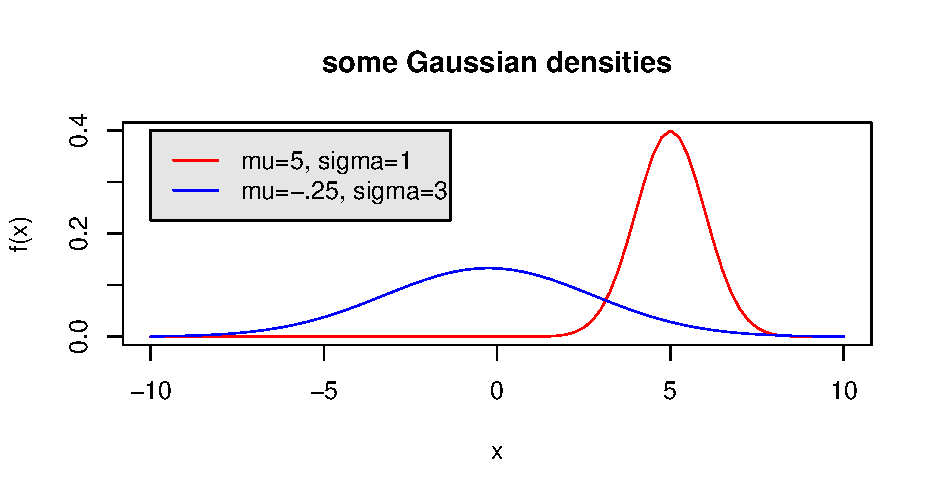
\includegraphics[width=100mm]{/home/taylor/UVa/all_teaching/3120_slides/3/3.7/pics/Rplot.pdf}
% \end{center}
% 
% \end{frame}

%----------------------------------------------------------------------------------------

\end{document} 